\chapter{光子与声子}\label{ch:b3:photons-phonons}

量子理论正是诞生于本章所述的主题之中。1900 年，
发光物体的光谱拒绝服从经典物理的描述——
更糟的是，经典理论预言短波长处的能量为\emph{无穷大}，
即所谓的“紫外灾难”——而普朗克那出于无奈的补救办法，
即能量以 $h\nu$ 为单位成包传递，结果成了本世纪的
关键钥匙。有了现已建立的工具——模式
计数（来自\cref{ch:b3:schrodinger-three-dimensions}），振子
热力学（来自\cref{ch:b3:canonical-ensemble}）——普朗克定律
只需半页篇幅即可导出：一团光子气体，每个
腔模对应一个玻色占据的振子。同样这半页篇幅，若以声音代替光，
便是德拜的固体理论，即爱因斯坦模型未能给出的 $T^3$ 热容。
而充满宇宙每一立方厘米空间的，则是本学科的杰作：
2.725 开尔文的宇宙微波
背景，是迄今测得最完美的\omterm{thm:b3:photons-phonons:planck}{黑体辐射}——
年轻宇宙自身的热辐射，至今仍在抵达我们。

\section{普朗克定律的推导}

\begin{theorem}[黑体辐射谱]\label{thm:b3:photons-phonons:planck}
\index{普朗克定律}\index{黑体辐射}
温度为 $T$ 的空腔中存在电磁模式——
驻波，其计数方法与
\cref{prop:b3:schrodinger-three-dimensions:counting} 完全相同，
但偏振方向须计两次：
\[
g(\nu)\,\dd\nu = \frac{8\pi V}{c^3}\,\nu^2\,\dd\nu .
\]
每个模式都是一个量子振子，平衡时含有
$\bar n = 1/(\eu^{h\nu/k_{\text{B}}T} - 1)$ 个光子
（见\cref{exo:b3:canonical-ensemble:5}；等价地，玻色子取 $\mu =
0$ 的情形）。单位体积、单位频率的能量因此为
\[
u(\nu, T) = \frac{8\pi h\nu^3}{c^3}\,
\frac{1}{\eu^{h\nu/k_{\text{B}}T} - 1} :
\]
\emph{普朗克定律}（1900 年）。其各项结论均与测量相符：
峰值位于 $\lambda_{\max}T = \qty{2898}{\micro m.K}$ 处（维恩
位移定律，即本科二年级分册中的内容，现已导出）；黑体表面的总通量
$\Phi = \sigma T^4$，其中
\[
\sigma = \frac{2\pi^5k_{\text{B}}^4}{15h^3c^2}
 = \qty{5.67e-8}{W.m^{-2}.K^{-4}}
\]
（斯特藩–玻尔兹曼，其常数现由 $h$、$c$、
$k_{\text{B}}$ 构成）；光子数密度为 $n_\gamma \approx
\num{2.03e7}\,(T/\unit{K})^3$ 每立方米。
\end{theorem}

\begin{proof}[部分证明]
将模式计数乘以 $h\nu\,\bar n$。总能量
积分取 $x = h\nu/k_{\text{B}}T$，并利用 $\int_0^\infty
x^3\dd x/(\eu^x - 1) = \pi^4/15$（承认），得 $u_{\text{总}}
= aT^4$，再乘以标准通量因子 $c/4$，即得
所述的 $\sigma$。维恩定律即
\cref{exo:b3:photons-phonons:1} 中的极大化。低频时（$h\nu \ll
k_{\text{B}}T$）每个模式携带的能量为 $k_{\text{B}}T$——
瑞利–金斯公式适用于无线电波段，若推广到所有
$\nu$，则会导致灾难。普朗克的截断，就是对能量均分的
许可（\cref{thm:b3:canonical-ensemble:equipartition}）的撤销，
逐个模式地进行。
\end{proof}

\begin{omfigure}
\begin{tikzpicture}
  \begin{axis}[omaxis, axis x line=bottom, axis y line=left,
    width=11.4cm, height=6.0cm, xmin=0, xmax=4.4, ymin=0, ymax=1.5,
    xlabel={$\nu$（单位：$10^{14}$ Hz）}, ylabel={$u(\nu)$（归一化）},
    xlabel style={at={(axis description cs:0.5,-0.09)}, anchor=north},
    xtick={1,2,3,4}, ytick=\empty, clip=false,
    legend style={font=\scriptsize, at={(0.97,0.93)}, anchor=north east,
      draw=none, fill=none}]
    \addplot[omDef, very thick, domain=0.01:4.4, samples=200]
      {1.42*x^3/(exp(x/1.208)-1)/8.3};
    \addlegendentry{$T = \qty{5800}{K}$（太阳）}
    \addplot[omThm, thick, domain=0.01:4.4, samples=200]
      {1.42*x^3/(exp(x/0.833)-1)/2.72};
    \addlegendentry{$T = \qty{4000}{K}$}
    \addplot[omExo, thick, domain=0.01:4.4, samples=200]
      {1.42*x^3/(exp(x/0.625)-1)/1.15};
    \addlegendentry{$T = \qty{3000}{K}$}
    \addplot[gray, dashed, domain=0.01:1.9, samples=100]
      {1.42*x^2*1.208/8.3};
    \node[gray, font=\scriptsize, anchor=west, rotate=48] at (axis cs:1.28,0.62)
      {瑞利–金斯};
  \end{axis}
\end{tikzpicture}

{\small 三种温度下的普朗克谱（各曲线已缩放至
相近高度，真实面积按 $T^4$ 增长）。经典的
瑞利–金斯线沿低频一侧延伸，随后
向紫外灾难方向急剧上升；普朗克的 $h\nu$ 代价
切断高频模式，使曲线向下弯。}
\end{omfigure}

\begin{example}[三支温度计]\label{ex:b3:photons-phonons:thermometers}
太阳（$T = \qty{5800}{K}$）：峰值位于 \qty{0.50}{\micro m}——
我们的眼睛恰好进化到对准它的峰值。温度为 \qty{310}{K} 的物体：峰值
位于 \qty{9.4}{\micro m} 附近，每平方米皮肤辐射 $\sigma T^4 \approx
\qty{520}{W/m^2}$ 的功率（所幸房间也会向外
辐射回去；
见\cref{exo:b3:photons-phonons:2}）。宇宙（$T =
\qty{2.725}{K}$）：峰值在 \qty{1.9}{mm} 附近（以频率表示为
\qty{160}{GHz}），每立方厘米 $411$ 个光子——
即宇宙微波背景，这是本章的重要范例
（\cref{pb:b3:photons-phonons:1}）。
\end{example}

\begin{proposition}[光的热力学]\label{prop:b3:photons-phonons:thermo}
\index{辐射压强!热}
光子气体的能量密度为 $u = aT^4$（$a =
4\sigma/c$），压强
\[
P = \frac u3 ,
\]
熵密度为 $\tfrac43 aT^3$，光子数 $\propto T^3$。
推论：绝热膨胀的充满辐射的箱子
按 $T \propto 1/L$ 降温——膨胀宇宙的光子
从 $3000$ K 冷却到今天的 $2.725$ K，膨胀因子
为 $\approx1100$，同时\emph{保持}完美的普朗克谱；并且
在大质量恒星中，$T^4$ 的增长使辐射压强可与
气体压强相抗衡，从而为恒星质量设定上限
（见\cref{ch:b3:astrophysics}）。
\end{proposition}

\begin{proof}[部分证明]
$P = u/3$：速率为 $c$ 的各向同性粒子气体，
将其能量密度的三分之一作为压强输出（因子 $\langle
\cos^2\theta\rangle = 1/3$，见本科一年级分册中的动理论）。
由 $\dd U = T\dd S - P\dd V$ 得熵，代入 $U =
aT^4V$。绝热时 $S \propto T^3V$ 为常数，故 $T \propto
V^{-1/3}$。
\end{proof}

\section{声子：德拜的完善}

\begin{theorem}[德拜模型]\label{thm:b3:photons-phonons:debye}
\index{德拜模型}\index{声子}
晶体的振动是\omterm{prop:b3:continuum-elasticity:waves}{弹性波}，其量子化方式与
光完全相同：\emph{声子}，三种偏振，声速为
$c_{\text{s}}$，按光子的方式计数，但总数上限为
$3N$ 个模式——该上限定义了\emph{德拜温度}
\[
k_{\text{B}}\theta_{\text{D}} = \hbar c_{\text{s}}
(6\pi^2n)^{1/3} .
\]
热容在两条经典定律之间过渡：
\[
C \to 3Nk_{\text{B}} \;(T \gg \theta_{\text{D}})
\qquad\text{（杜隆–珀蒂）} ,
\qquad
C \to \frac{12\pi^4}{5}\,Nk_{\text{B}}
\Big(\frac{T}{\theta_{\text{D}}}\Big)^3
\;(T \ll \theta_{\text{D}}) :
\]
低温量热测量所要求的 $T^3$ 定律，而
爱因斯坦的单一频率无法给出
（见\cref{exo:b3:canonical-ensemble:6}）。其原因与
光的情形相同：无论晶体多冷，总存在任意廉价的
长波长声子，其类光子的计数方式
给出类光子的 $T^3$ 规律。
\end{theorem}

\begin{proof}[部分证明]
将光子的计算重做一遍，取 $c \to c_{\text{s}}$、三种
偏振，并由模式总数 $\int g\,\dd\nu = 3N$ 确定
截止频率。在 $T \ll \theta_{\text{D}}$ 时，截止
$T^4$ 的能量积分给出 $C \propto T^3$；在高 $T$ 时，
$3N$ 个模式中的每一个都携带 $k_{\text{B}}T$。完整的
插值积分在本阶段不加证明地承认。
\end{proof}

\begin{omfigure}
\begin{tikzpicture}
  \begin{axis}[omaxis, axis x line=bottom, axis y line=left,
    width=11.0cm, height=5.6cm, xmin=0, xmax=1.5, ymin=0, ymax=1.15,
    xlabel={$T/\theta_{\text{D}}$}, ylabel={$C/3Nk_{\text{B}}$},
    xlabel style={at={(axis description cs:0.5,-0.1)}, anchor=north},
    xtick={0.5,1,1.5}, ytick={0.5,1}, clip=false,
    legend style={font=\scriptsize, at={(0.95,0.42)}, anchor=north east,
      draw=none, fill=none}]
    \addplot[gray, dashed, domain=0:1.5, forget plot] {1};
    \addplot[omDef, very thick, domain=0.02:1.5, samples=200]
      {1/(1+0.01283/(x*x*x))};
    \addlegendentry{德拜}
    \addplot[omExo, thick, dashed, domain=0.02:1.5, samples=200]
      {(0.75/x)^2*exp(-0.75/x)/(1-exp(-0.75/x))^2};
    \addlegendentry{爱因斯坦}
    \node[omDef, font=\scriptsize, anchor=west] at (axis cs:0.2,0.28)
      {$\propto T^3$};
    \draw[->, omDef] (axis cs:0.2,0.24) -- (axis cs:0.13,0.13);
  \end{axis}
\end{tikzpicture}

{\small 晶体的热容：两个模型都趋于
杜隆–珀蒂定律，但在低温下爱因斯坦的单频曲线
指数衰减，而德拜的廉价长波声子
维持实测的 $T^3$ 规律，低 $T$ 区是纯粹的
“光子物理”借声音实现。}
\end{omfigure}

\begin{example}[声子是真实的粒子]\label{ex:b3:photons-phonons:phonon-real}
声子与中子、X 射线的散射满足能量与（晶体）
动量守恒——实测色散曲线
$\omega(\vect k)$（见\cref{ch:b3:crystalline-solids}）正是它们的
光谱学。它们还携带热量：绝缘体的热导率
为声子气体的 $\kappa = \tfrac13 Cc_{\text{s}}\ell$，而
金刚石——坚硬、轻质、纯净——在室温下的热导率
仅凭声子便为铜的五倍
（见\cref{exo:b3:photons-phonons:12}）。它们在低温下
按 $T^3$ 的规律消失，这正是低温工程师称晶体
“声学沉寂”的原因。
\end{example}

\begin{method}[辐射气体方法]\label{met:b3:photons-phonons:method}
(1) 计数模式（三维中每种偏振的模式数 $\propto\nu^2$）；以
$1/(\eu^{\beta h\nu} - 1)$ 作占据数；积分，预期能量为 $T^4$，
计数与热容为 $T^3$。(2) 峰值由维恩定律给出；
总量由斯特藩定律给出；每模式的经典值 $k_{\text{B}}T$ 只在
$h\nu \sim k_{\text{B}}T$ 以下成立。(3) 对固体，将模式截断于 $3N$
（$\theta_{\text{D}}$）；光学支模式用爱因斯坦形式，
声学支用德拜形式。(4) 绝热辐射：$T \propto
V^{-1/3}$。(5) 核对两个常用常数：$\lambda_{
\max}T = \qty{2898}{\micro m.K}$ 和 $\sigma =
\qty{5.67e-8}{W/m^2K^4}$。
\end{method}

\begin{omfigure}
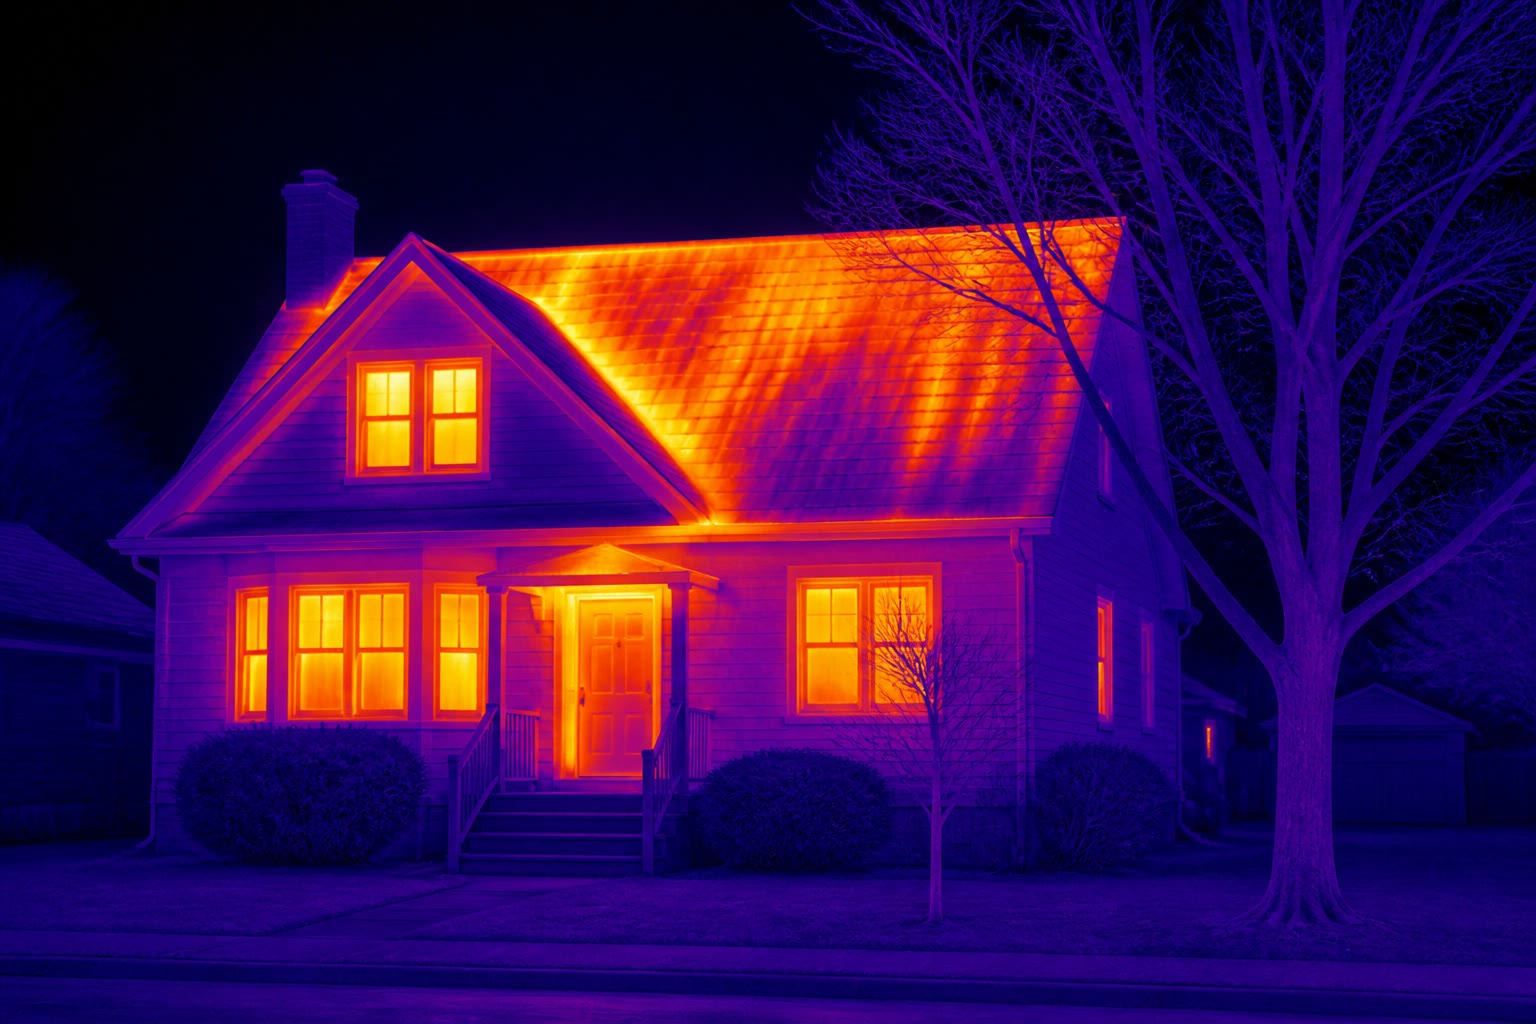
\includegraphics[width=0.58\linewidth]{images/book5/ai/b5-09-thermal-house.jpg}

{\small 透过热像仪看到的一座房屋：每个表面都辐射其普朗克谱，相机直接从红外线读出温度——斯特藩、玻尔兹曼与维恩正在为供暖账单做审计。}
\end{omfigure}

\section{练习}

\begin{exercise}[$\star$]\label{exo:b3:photons-phonons:1}
(a) 由波长形式的普朗克定律证明峰值满足
$\lambda_{\max}T = $ 为常数（可引用超越方程
$x = 4.965$）。(b) 求峰值波长，对象为
太阳、\qty{2700}{K} 灯丝、\qty{310}{K} 物体和
\qty{2.725}{K} 天空。(c) 四者中哪一个能被人眼较好地感知？
灯丝辐射中可见部分占多大比例（估算：很小）？
(d) 为何“红外照相机”
是测量人与建筑的合适工具？
\end{exercise}

\begin{exercise}[$\star$]\label{exo:b3:photons-phonons:2}
辐射收支。(a) 一人（面积 $\qty{1.7}{m^2}$，皮肤
温度 \qty{306}{K}），位于 \qty{293}{K} 的房间中：净辐射功率
$\sigma A(T_1^4 - T_2^4)$。(b) 与人体的
\qty{100}{W} 代谢率相比，为何我们仍能忍受（衣着，以及房间的回辐射）？
(c) 地球吸收太阳光的面积为 $\pi
R^2$，辐射面积为 $4\pi R^2$：推导 $T_{\text{有效}}
= [(1-A)\,\Phi_\odot/4\sigma]^{1/4}$，其中 $\Phi_\odot =
\qty{1361}{W/m^2}$，反照率 $A = 0.30$，并求值。(d) 实测
地表平均温度为 \qty{288}{K}，请指出
\qty{33}{K} 温差的机制
（见\cref{pb:b3:harmonic-oscillator:1}）。
\end{exercise}

\begin{exercise}[$\star$]\label{exo:b3:photons-phonons:3}
光子计数。(a) 取 $n_\gamma = \num{2.03e7}\,T^3$，
求 \qty{2.725}{K} 背景辐射的光子数密度（单位为每立方米）。
(b) 地球处的太阳光：由 $\Phi_\odot$ 及平均光子能量
$\approx 2.7\,k_{\text{B}}T_\odot \approx \qty{1.35}{eV}$，
求每平方米每秒的光子通量。(c) 一只
\qty{60}{W} 白炽灯（可见光占 5\%）的
每秒可见光子数。(d) 为何“光子计数”对天文学家是常规，
而对取暖器却荒谬？
\end{exercise}

\begin{exercise}[$\star$]\label{exo:b3:photons-phonons:4}
紫外灾难及其尾部。(a) 证明经典能量均分
（每个模式 $k_{\text{B}}T$）给出 $u(\nu) =
8\pi\nu^2k_{\text{B}}T/c^3$，积分时发散。(b) 普朗克定律在何处
退化为该式？(c) 射电天文学家测量
\qty{1.4}{GHz} 处的宇宙微波背景：验证其中 $h\nu/k_{\text{B}}T \ll 1$，
并说明他们习惯以“天线温度”为名，
用开尔文给出强度的理由。(d) 在宇宙微波背景的 \qty{160}{GHz} 峰值处求
$h\nu/k_{\text{B}}T$，该峰值是否属于经典情形？
\end{exercise}

\begin{exercise}[$\star\star$]\label{exo:b3:photons-phonons:5}
辐射压强。(a) 由各向同性推导 $P = u/3$（或接受
动理学因子），并求地球轨道处太阳光的压强，
与大气压强相比。(b) 在太阳内部
（$T \approx \qty{1.5e7}{K}$）计算 $P_{\text{辐射}} =
aT^4/3$，并与气体压强 $\sim\qty{2e16}{Pa}$ 相比较。
(c) 辐射压强随 $T^4$ 增长，气体压强随 $T$ 增长：说明
为何质量足够大（因而更热）的恒星
会由辐射主导而不稳定——即爱丁顿极限，约在
$\sim100\,M_\odot$ 附近。(d) 激光：一束 \qty{1}{kW} 光束聚焦后
用以推动物体——能产生多大的力？为何“牵引光束”只见于电影中，
而\emph{光镊}（依靠梯度力，皮牛顿量级）却是真实的工具？
\end{exercise}

\begin{exercise}[$\star\star$]\label{exo:b3:photons-phonons:6}
宇宙的膨胀。宇宙微波背景发出于复合时期
（$T \approx \qty{3000}{K}$，与\cref{exo:b3:grand-canonical:12}
所述情形相近），并以 \qty{2.725}{K} 抵达。(a) 由 $T \propto
1/a$，求自发射以来所有长度的尺度因子。(b) 证明
普朗克谱在各波长被均匀伸展后
仍为普朗克谱（$T$ 如何变化？）。(c) 发出的峰值（可见的
橙光！）抵达时位于何处？(d) 为何天空对人眼来说是暗的，
而对微波接收机却十分明亮？
\end{exercise}

\begin{exercise}[$\star\star$]\label{exo:b3:photons-phonons:7}
由声速求德拜温度。(a) 计算 $\theta_{\text{D}} =
\hbar c_{\text{s}}(6\pi^2n)^{1/3}/k_{\text{B}}$，取铜的
（$c_{\text{s}} \approx \qty{3800}{m/s}$，$n =
\qty{8.5e28}{m^{-3}}$），并与量热测得的
\qty{343}{K} 作比较。(b) 金刚石：$c_{\text{s}} \approx
\qty{13000}{m/s}$，$n = \qty{1.76e29}{m^{-3}}$：求值，
并与 $\approx\qty{2200}{K}$ 比较。(c) 铅：柔软而沉重——
用一句话解释其 $\theta_{\text{D}} \approx \qty{90}{K}$
的原因。(d) 给出联系固体刚度、
原子质量与其量子凝固温度的规律。
\end{exercise}

\begin{exercise}[$\star\star$]\label{exo:b3:photons-phonons:8}
一开尔文下的铜。(a) 利用 $C = \gamma T + \beta T^3$，其中
$\gamma$ 取自\cref{ex:b3:quantum-statistics:heat}，德拜
$T^3$ 项系数（$\theta_{\text{D}} = \qty{343}{K}$），求
两项在 \qty{1}{K} 时每摩尔的值。(b) 哪一项占优，
优势多大？(c) 两项在何温度处相等？(d) 为何这一区间是量热学家
借以观察电子
\omterm{prop:b3:schrodinger-three-dimensions:counting}{态密度}的窗口？
\end{exercise}

\begin{exercise}[$\star\star$]\label{exo:b3:photons-phonons:9}
单层温室。设表面（温度 $T_s$）位于
一层薄大气层（温度 $T_a$）之下，该层对
太阳光透明而对热红外线不透明。(a) 分别写出该层的能量平衡
（吸收 $\sigma T_s^4$，辐射
$2\sigma T_a^4$）与表面的能量平衡（吸收太阳光 $S$ 加
$\sigma T_a^4$）。(b) 证明 $T_s = 2^{1/4}\,T_{\text{有效}}$，其中
$\sigma T_{\text{有效}}^4 = S$。(c) 取 $T_{\text{有效}} =
\qty{255}{K}$，求 $T_s$ 并与 \qty{288}{K} 比较
（真实大气层是部分透明的多层“毯子”）。(d)
结合\cref{pb:b3:harmonic-oscillator:1}，
哪种分子物理使该层在红外线中不透明，而在
可见光中透明？
\end{exercise}

\begin{exercise}[$\star\star\star$]\label{exo:b3:photons-phonons:10}
从头推导斯特藩常数。(a) 组装 $u_{\text{总}} =
\int u(\nu)\dd\nu$，取 $x = h\nu/k_{\text{B}}T$，并利用给定的
$\pi^4/15$，得 $u = aT^4$，其中 $a =
8\pi^5k_{\text{B}}^4/15h^3c^3$。(b) 黑体
表面的通量为 $c\,u/4$（取几何因子四分之一）：写出
$\sigma$，并由 $h$、$c$、
$k_{\text{B}}$ 数值求值。(c) 与 \qty{5.67e-8}{W.m^{-2}.K^{-4}} 比较。
(d) 历史回顾：普朗克于 1900 年用他的定律拟合光谱，
并提取出\emph{两者}：$h$ 和 $k_{\text{B}}$（进而得到阿伏伽德罗
常数）——说明黑体曲线为何能同时确定两个
常数。
\end{exercise}

\begin{exercise}[$\star\star\star$]\label{exo:b3:photons-phonons:11}
爱因斯坦的 A 与 B（1917）。两能级原子（能量 $0,
h\nu_0$；粒子数 $N_1, N_2$）处于谱密度为
$u(\nu_0)$ 的辐射中。吸收速率：$B_{12}uN_1$；受激辐射：
$B_{21}uN_2$；自发辐射：$AN_2$。(a) 写出
平衡态下的收支方程。(b) 要求玻尔兹曼比
$N_2/N_1 = \eu^{-h\nu_0/k_{\text{B}}T}$ 与普朗克的 $u$
对\emph{所有} $T$ 同时成立，由此推出 $B_{12} = B_{21}$ 以及
\[
\frac{A}{B} = \frac{8\pi h\nu_0^3}{c^3} .
\]
(c) 解释：热平衡为何\emph{必然}要求存在自发辐射，
并由受激辐射确定其速率？
(d) 关于 $\nu^3$：结合
\cref{exo:b3:perturbation-theory:8}中的寿命，
说明为何在 X 射线频段实现激光十分困难。
\end{exercise}

\begin{exercise}[$\star\star\star$]\label{exo:b3:photons-phonons:12}
金刚石，声子的超级高速公路。绝缘体的热导率
为 $\kappa = \tfrac13 C_v c_{\text{s}}\ell$（单位体积），其中
$\ell$ 为声子平均自由程。(a) 对于金刚石，取
\qty{300}{K}（$C_v \approx \qty{1.8e6}{J.m^{-3}K^{-1}}$，即部分“冻结”；
$c_{\text{s}} = \qty{13000}{m/s}$；$\ell
\approx \qty{0.3}{\micro m}$）：计算 $\kappa$，并与
铜的 \qty{400}{W/(m.K)} 比较。(b) 为何金刚石中的 $\ell$ 如此之长
（刚性大、质量轻、同位素纯净——什么会散射声子？）。
(c) 同位素提纯使金刚石的 $\kappa$ 几乎翻倍：这说明
声子被同位素质量无序散射说明了什么？
(d) 两种用途：电子器件中的散热片；以及为何
金刚石贴近嘴唇时会有冰凉感——解释这种感觉。
\end{exercise}

\begin{omfigure}
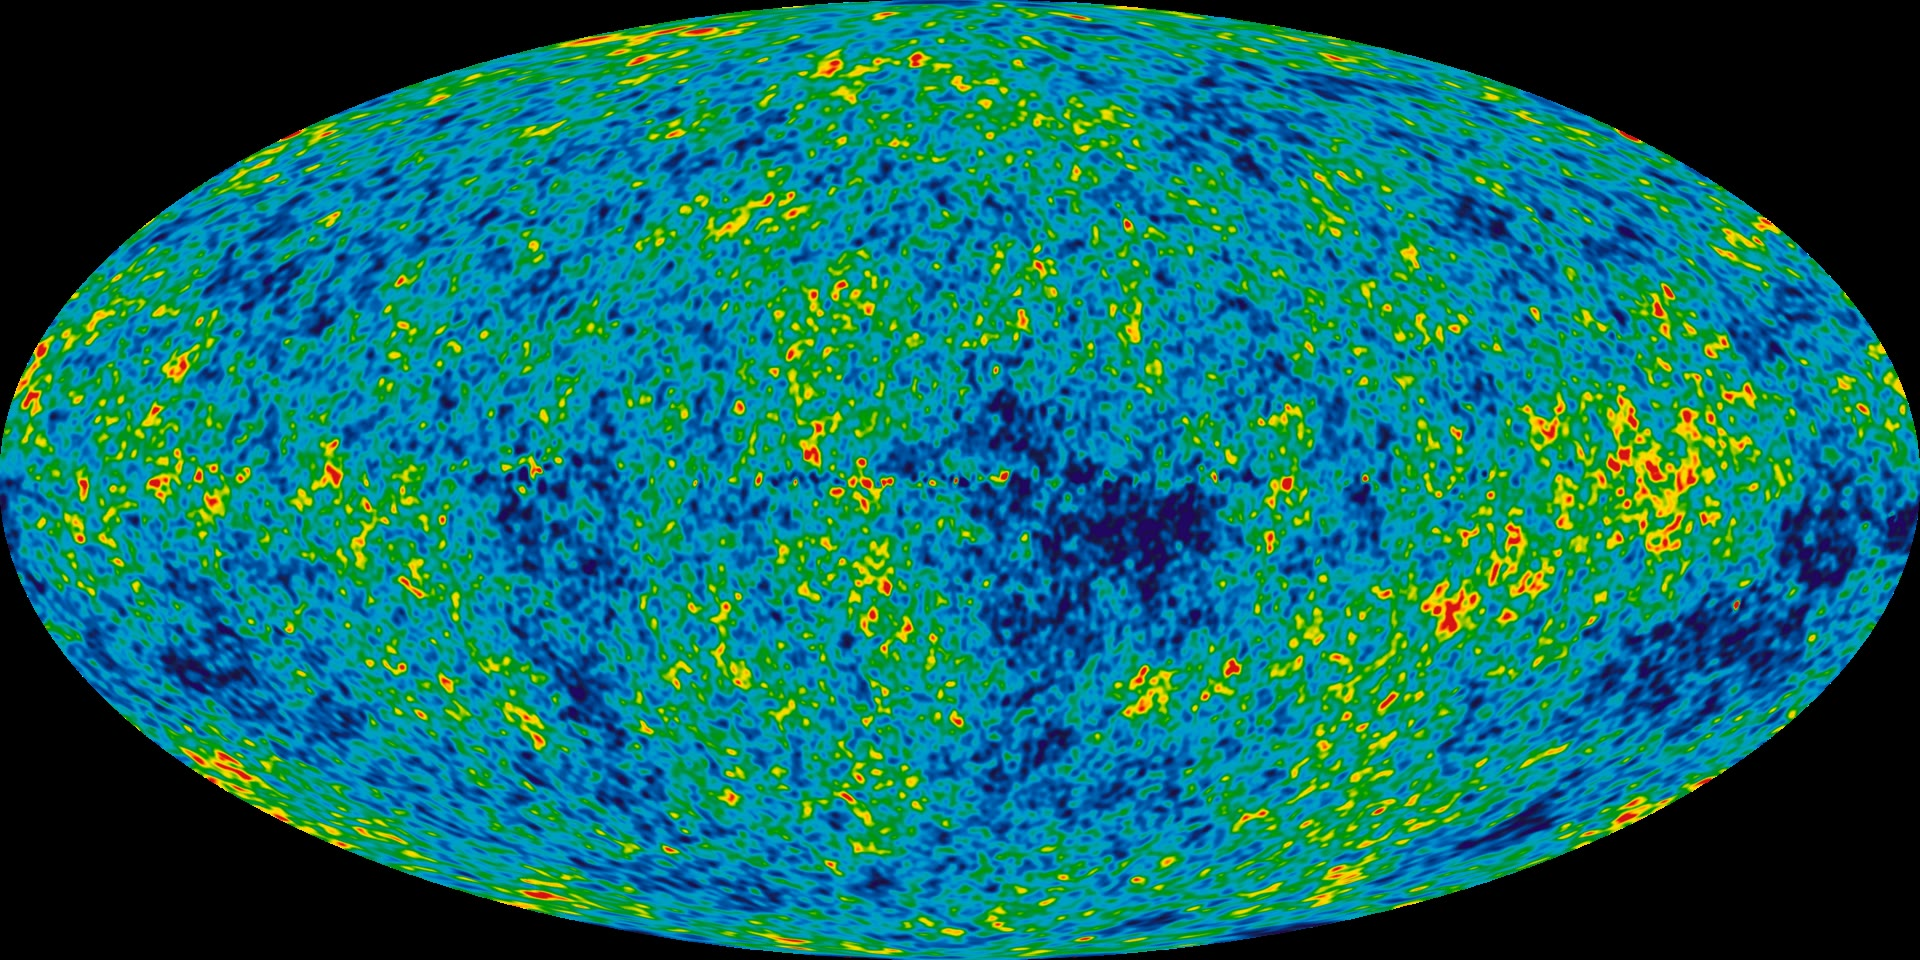
\includegraphics[width=0.62\linewidth]{images/book5/photo-cmb-wmap.jpg}

{\small 微波下的全天图（NASA/WMAP，公有领域）：宇宙背景的 \qty{2.7}{K} 普朗克辐射，经测绘而成。斑驳起伏仅为 $10^5$ 分之一——星系的种子，印在本章的黑体谱上。}
\end{omfigure}

\section{问题：最古老的光}

\begin{problem}[{周末问题——读取宇宙
微波背景}]\label{pb:b3:photons-phonons:1}
将任一毫米波接收器对准天空的任一区域，它都会
报告相同的信号：温度为 $T =
\qty{2.72548(57)}{K}$ 的普朗克谱，比人类所
造的任何炉子都更平滑。它是宇宙复合时刻的
闪光（见\cref{exo:b3:grand-canonical:12}），被拉伸了约一千一百倍，
并记录着宇宙的全部普查信息。数据：$T_0 =
\qty{2.725}{K}$；$n_\gamma = \num{2.03e7}\,T^3\,\unit{m^{-3}}$；
$u = aT^4$，$a = \qty{7.56e-16}{J.m^{-3}.K^{-4}}$；今日重子数密度
$n_{\text{b}} \approx \qty{0.25}{m^{-3}}$；临界密度
$\rho_{\text{c}} \approx \qty{8.6e-27}{kg/m^3}$。

\medskip\noindent\textbf{第一部分——光谱。}
\begin{enumerate}
  \item 计算宇宙微波背景的峰值（维恩）波长及其光子
        数密度（以每立方厘米计）。
  \item 计算其能量密度，分别以 $\unit{J/m^3}$ 和
        $\unit{eV/cm^3}$ 为单位，并求其质量当量占
        临界密度的比例。
  \item COBE 的光谱（1990 年）与普朗克谱吻合到约
        $10^4$ 分之几——观众为这张图鼓掌。为何来自空无一物的天空的
        \emph{完美热}光谱，
        除了炽热致密的过去，几乎无法用其他任何东西解释？
  \item 发射时，这些光子构成一个 \qty{3000}{K}
        黑体：检验拉伸因子 $1 + z =
        T_{\text{当时}}/T_0$。
  \item 为何宇宙恰在该温度下变得透明（回忆
        哪种平衡在
        \cref{ch:b3:grand-canonical} 中被关闭）？
  \item 夜空是暗的（旧天文学中的奥伯斯佯谬）：它在何种确切意义上
        实际是
        \emph{明亮}的——在什么波长与温度下？
\end{enumerate}

\medskip\noindent\textbf{第二部分——普查。}
\begin{enumerate}[resume]
  \item 计算光子与重子之比 $\eta^{-1} =
        n_\gamma/n_{\text{b}}$。
  \item 这一数字——每个质子约对应二十亿个光子——
        是宇宙学的基本数据之一：说明它度量的是
        物质—反物质不对称的什么信息（回忆
        \cref{exo:b3:grand-canonical:12}：光子大多是
        湮灭产物）。
  \item 比较宇宙微波背景与星光的能量密度
        （对整个宇宙平均约为 $\sim\qty{2e-15}{J/m^3}$）：
        哪种光主导着宇宙？
  \item 按光子数计，宇宙微波背景超过了恒星曾经发出的全部光：
        为何这使早期宇宙成为“辐射主导”的，
        随后又是什么取而代之（
        $T^4$ 与 $T^3$ 的标度，对比物质的 $a^{-3}$）？
  \item 估算物质—辐射相等的时代：辐射密度按 $(1+z)^4$ 标度，
        物质密度按 $(1+z)^3$ 标度，
        且今日比值
        $u_{\text{辐射}}/\rho_{\text{m}}c^2 \approx 1/3400$，求
        $z_{\text{平衡}}$。
  \item 中微子更早退耦，降温稍多（它们错过了
        $e^+e^-$ 湮灭的再加热，见
        \cref{exo:b3:grand-canonical:12}）：预言的
        $T_\nu = (4/11)^{1/3}T_\gamma$——计算它，并惊叹于
        对一个 \qty{1.95}{K} 中微子海的预言，
        而这中微子海至今尚无人直接探测到。
\end{enumerate}

\medskip\noindent\textbf{第三部分——各向异性。}
\begin{enumerate}[resume]
  \item 宇宙微波背景在一个方向上高 \qty{3.4}{mK}，在相反方向上则低相同的量：
        借助
        \cref{ch:b3:relativistic-kinematics}中的多普勒物理加以解释，并由此求出我们的
        速度（$\Delta T/T = v/c$）。
  \item 去掉这一偶极项后，仍残留 $\Delta T/T \sim
        \num{e-5}$ 的起伏（COBE 1992 年，随后是 WMAP、普朗克）：
        它们在 $z = 1100$ 处映射的是什么？
  \item 这些 $10^{-5}$ 的密度种子长成了星系：为什么
        引力会放大过密区（属于哪种不稳定性），
        而增长为何需要物质–辐射相等，
        才真正开始？
  \item 最强起伏的尺度（天空中约一度）
        是一个声学波长——即光子–重子等离子体中的声音（本章的气体
        加上
        \cref{ch:b3:continuum-elasticity}中的波！）：是什么决定了它的尺度
        （即
        复合之前声音所传播的距离）？
  \item 将该角度与已知的物理尺度相比较，
        即可三角测量出宇宙的几何：给出结果
        （平坦的，精确到百分之几）。
  \item 请为 \qty{2.7}{K} 的单极项、\qty{3}{mK} 的偶极项、
        \num{e-5} 的起伏所教给我们的东西排序（炽热的过去；
        我们的运动；一切的种子与几何）。
\end{enumerate}

\medskip\noindent\textbf{第四部分——遗产。}
\begin{enumerate}[resume]
  \item 1965 年，彭齐亚斯与威尔逊发现了这一信号，
        它被当作无法消除的天线噪声（在赶走了鸽子之后）：
        为什么一个\emph{各向同性}、与季节无关的超额，
        在 \qty{3}{K} 处无法被解释为任何局域或银河系的源？
  \item 未调谐的模拟电视雪花噪声中，约有 $1\%$
        来自这一信号：用一句话加以说明。
  \item 宇宙微波背景穿过星系团，
        被热电子略微推向更高频率（即苏尼亚耶夫–泽尔多维奇效应）：
        为什么这使得星系团在低频下
        表现为\emph{阴影}，
        而这种阴影的特殊优点是什么
        （与距离无关）？
  \item 当今的前沿工作在宇宙微波背景的偏振中寻找
        原初引力波留下的印记：这一发现会把本书的哪些章节
        联系在一起？
        （\cref{ch:b3:covariant-electromagnetism}中的偏振，
        以及引力波）？
  \item 计算宇宙微波背景光子穿过你身体的通量
        （单位面积上为 $n_\gamma c/4$，人体\omterm{def:b3:scattering-theory:cross-section}{截面}
        $\sim\qty{0.5}{m^2}$）：
        每秒有多少个大爆炸的遗迹穿过你？
  \item 宇宙微波背景确定了一个静止参考系（即偶极项消失的那个参考系）：
        请解释为什么这\emph{并不}
        与相对论相矛盾——这一参考系是由
        物质成分而非定律所选定的，它属于哪一类参考系？
  \item 概括这一著名结果：一条 $2.725$ 开尔文的普朗克曲线
        充满天空——每立方厘米 $411$ 个光子，
        每个重子对应二十亿个光子，峰值位于
        \qty{160}{GHz}——它是炽热开端的热学回执：
        统计物理是宇宙学的
        基石。
\end{enumerate}
\end{problem}
